\documentclass[11pt,a4paper]{article}
\usepackage[utf8]{inputenc}
\usepackage[T1]{fontenc}
\usepackage{microtype}
\usepackage{geometry}
\usepackage{hyperref}
\usepackage{enumitem}
\usepackage{listings}
\usepackage{xcolor}
\usepackage{tikz}
\usetikzlibrary{shapes.geometric, arrows.meta, positioning}

\geometry{margin=1in}

% Code listing style
\lstset{
  basicstyle=\ttfamily\small,
  breaklines=true,
  frame=single,
  backgroundcolor=\color{gray!10},
}

\title{Emo Dataset Verifier: Approach and Methodology}
\author{}
\date{}

\begin{document}

\maketitle

\section{Overview}

The emo dataset verifier (\texttt{verify\_emo\_dataset.py}) identifies hand-labeled emo tracks that may be mislabeled---i.e., tracks in \texttt{emo/} that are actually non-emo. Because we cannot listen to audio programmatically, the verifier uses two complementary statistical methods to flag candidates for manual review.

\section{Problem Statement}

Training data quality directly affects classifier accuracy. If non-emo tracks are placed in \texttt{emo/}, the model learns incorrect patterns and produces more false positives. The verifier helps surface potential mislabels so a human can listen and correct them.

\section{Method 1: Local Outlier Factor (LOF)}

\subsection{Idea}

Emo music shares certain acoustic characteristics (e.g., guitar-driven, dynamic range, typical tempo and timbre). Tracks labeled emo that differ strongly from the emo cluster in feature space may be mislabeled.

\subsection{How It Works}

\begin{enumerate}
  \item \textbf{Features}: For each emo sample, we extract Librosa audio features (MFCC, chroma, spectral centroid, rolloff, bandwidth, zero-crossing rate, RMS energy, tempo).
  \item \textbf{Space}: We build a feature matrix of all emo samples only (no non-emo).
  \item \textbf{LOF}: We fit \texttt{LocalOutlierFactor} on this emo-only feature space. LOF assigns each sample an ``outlier score.''
  \item \textbf{Selection}: Samples with the most negative scores are the strongest outliers---their audio features diverge the most from the typical emo cluster.
\end{enumerate}

\subsection{Interpretation}

\begin{itemize}
  \item \textbf{Outlier \(\neq\) guaranteed mislabel}. Outliers may be legitimately emo but stylistically different (e.g., acoustic emo vs.\ post-hardcore).
  \item \textbf{Outlier = worth checking}. These are the best candidates for manual listening and potential re-labeling.
\end{itemize}

\subsection{Parameters}

\begin{itemize}
  \item \texttt{n\_neighbors}: Set to \(\min(20, \lvert \text{emo} \rvert / 2)\) to adapt to dataset size.
  \item \texttt{n}: Top \(N\) most outlier-like emo samples are flagged (default 40).
\end{itemize}

\section{Method 2: Cross-Validation Misprediction}

\subsection{Idea}

If a model trained on most of the data repeatedly predicts an emo sample as ``Not Emo'' with high confidence, that sample may be mislabeled.

\subsection{How It Works}

\begin{enumerate}
  \item \textbf{Stratified K-Fold}: Split the full dataset (emo + not\_emo) into \(K\) folds while preserving class balance.
  \item \textbf{Per fold}: Train a RandomForest on \(K-1\) folds, predict on the held-out fold.
  \item \textbf{Focus on emo samples}: For each emo sample, record how often it was predicted ``Not Emo'' with emo probability below a threshold (e.g., 0.25).
  \item \textbf{Flagging}: Emo samples mispredicted in at least half of the folds are flagged.
\end{enumerate}

\subsection{Interpretation}

\begin{itemize}
  \item A track labeled emo but consistently predicted Not Emo suggests it matches the non-emo distribution in feature space.
  \item This method uses the learned boundary between emo and not\_emo, so it complements LOF (which uses only emo internal structure).
\end{itemize}

\subsection{Parameters}

\begin{itemize}
  \item \texttt{n\_splits}: 5 folds.
  \item \texttt{prob\_threshold}: Emo probability below 0.25 counts as a misprediction.
\end{itemize}

\section{Combining Both Methods}

The verifier takes the \textbf{union} of samples flagged by either method. A file can be flagged because:

\begin{enumerate}
  \item It is an outlier in the emo cluster (LOF), or
  \item It is often predicted as Not Emo in cross-validation (CV), or
  \item Both.
\end{enumerate}

The combined list is written to \texttt{data/audio\_verification\_report.txt} for manual review.

\section{Workflow}

\begin{center}
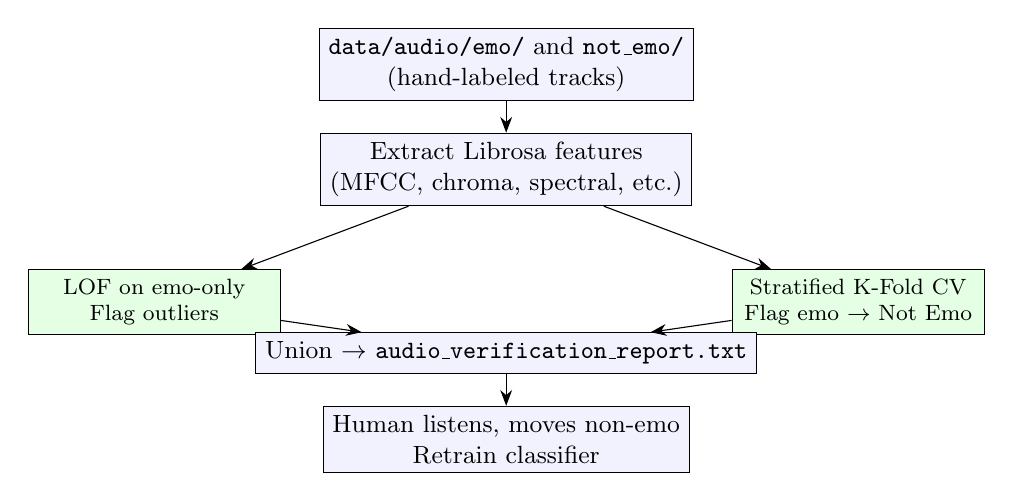
\begin{tikzpicture}[
  node distance=0.4cm,
  box/.style={rectangle, draw, fill=blue!5, minimum width=4.5cm, align=center, font=\small},
  smallbox/.style={rectangle, draw, fill=green!10, minimum width=3.2cm, align=center, font=\footnotesize},
  arrow/.style={-{Stealth[length=2mm]}}
]
  \node[box] (a) {\texttt{data/audio/emo/} and \texttt{not\_emo/}\\(hand-labeled tracks)};
  \node[box, below=of a] (b) {Extract Librosa features\\(MFCC, chroma, spectral, etc.)};
  \node[smallbox, below left=0.8cm and 0.5cm of b] (c) {LOF on emo-only\\Flag outliers};
  \node[smallbox, below right=0.8cm and 0.5cm of b] (d) {Stratified K-Fold CV\\Flag emo $\to$ Not Emo};
  \node[box, below=1.6cm of b] (e) {Union $\to$ \texttt{audio\_verification\_report.txt}};
  \node[box, below=of e] (f) {Human listens, moves non-emo\\Retrain classifier};

  \draw[arrow] (a) -- (b);
  \draw[arrow] (b) -- (c);
  \draw[arrow] (b) -- (d);
  \draw[arrow] (c) -- (e);
  \draw[arrow] (d) -- (e);
  \draw[arrow] (e) -- (f);
\end{tikzpicture}
\end{center}

\section{Limitations}

\begin{enumerate}
  \item \textbf{No ground truth}: We infer possible mislabels from statistics, not from listening.
  \item \textbf{Feature coverage}: Emo is partly defined by lyrics and emotional content, which Librosa features do not capture. Some mislabels may not be detected.
  \item \textbf{Edge cases}: Stylistically unusual but correct emo (e.g., slowcore, acoustic) may appear as outliers and be flagged.
  \item \textbf{Circularity in CV}: The model is trained on the same labels we are verifying. If many emo samples are mislabeled, the boundary is skewed and CV may miss some errors.
\end{enumerate}

\section{Usage}

\begin{lstlisting}[language=bash]
poetry run python -m verify_emo_dataset
\end{lstlisting}

Then:
\begin{enumerate}
  \item Open \texttt{data/audio\_verification\_report.txt}
  \item Listen to the listed files
  \item Move any confirmed non-emo files from \texttt{emo/} to \texttt{not\_emo/}
  \item Retrain: \texttt{poetry run python -m classifier\_audio}
\end{enumerate}

\section{References}

\begin{itemize}
  \item Breunig, M.\ M., Kriegel, H.-P., Ng, R.\ T., \& Sander, J.\ (2000). LOF: Identifying density-based local outliers. \textit{Proceedings of SIGMOD 2000}.
  \item McFee, B., et al.\ (2015). librosa: Audio and music signal analysis in Python. \textit{Proceedings of SciPy 2015}.
\end{itemize}

\end{document}
